\graphicspath{{./lab03/Images/}}


\maketitlepage{App Development}{in Android Studio}{Lab 3: Components}
\maketocpage


\section{Activities}
We have already used an activity without going into too much detail what it is. An activity is a single screen unit (usually full screen) with an user interface. So far we have only worked with a single activity but an Android app can have multiple activities. It breaks the app up into section with different purpose and UI. For example, a menu in an email app could be an activity while composing an email might be another, opened from the menu.\\

One activity serves as a luncher activity. It is our starting point when running the app (opposed to a C\texttt{++} main function) and from there on we can start navigating to other activities if any. Every app must have a luncher activity. All activities must be declared in our app's manifest\footnote{Android Studio does this automatically when an activity is created} and the luncher activity is also determined there.\\

Each activity uses a layout file that defines their UI at leat partially (some of it may be done dynamically in Java). In the \texttt{onCreate} function we have been setting the activity's layout with the \texttt{setContentView} method. Activities can share layouts although it serves a limited purpose unless most of the UI is dynamic. We will look at better ways to share UI in Fragments.\\

\subsection{Starting a new Activity}
Lets start by creating a new activity with \menu{File > New > Activity > Empty Activity} and name it \texttt{SecondActivity} and leave the other options as they are. Before proceeding you should inspect your manifest. Add a button to the luncher activity which calls the method \texttt{clicked()} upon being clicked and add some text to the second activity so it differentiates from the other one. Finally add the following method to the luncher activity and run the progam.

\begin{lstlisting}[style=A_Java]
public void clicked(View view) {
    startActivity(new Intent(MainActivity.this, SecondActivity.class));
}	
\end{lstlisting}

The \texttt{startActivity} method takes \texttt{Intent} as a paramter. We will look at that class, its parameters and methods in more detail later but for now, you can think of it as a bridge between two activities. 

\subsection{Lifecycle}
Activities are managed by a stack called the activity stack (or the back stack) and whatever activity is in our foreground is at the top of our stack. During the lifecycle of an activity, it can have various states and the event that brings us to set states have their own callback methods. This lifecycle can be seen in figure \ref{fig:actlife}.

\begin{figure}[H]
\centering
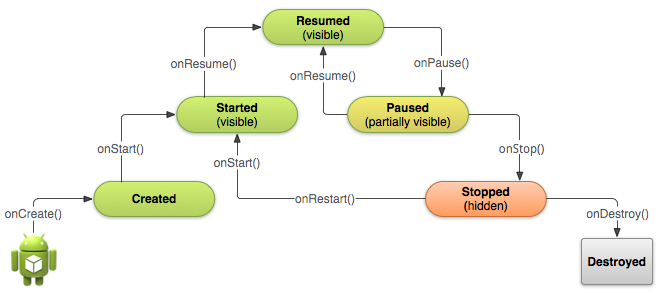
\includegraphics[scale=.5]{activity_state_machine.png}
\caption{The lifecycle of an Activity}
\label{fig:actlife}
\end{figure}

The states are
\begin{itemize}
	\item \textbf{Starting}. In the process of setting up.
	\item \textbf{Running}. In foreground.
	\item \textbf{Paused}. Not in foreground.
	\item \textbf{Stopped}. Inactive but remains in memory.
	\item \textbf{Destroyed}. Shut down and removed from memory.
\end{itemize}

There are multiple callback methods called when moving between states. We have already seen \texttt{onCreate} which is the only one that activities are required to override but there are several others.

\begin{itemize}
	\item \textbf{\texttt{onCreate()}}.\\
    \noindent This callback method is for the event of creating an activity and is called before the activity starts for the first time. It is typically used for initialization as we have been using it already.
	\item \textbf{\texttt{onStart()}}.\\
    \noindent Is called every time the activity starts, after entering the starting state. Here the activity becomes visible and prepares for entering the foreground and becoming interactive. This is where the app initializes the code that maintains the UI of the activity.
	\item \textbf{\texttt{onResume()}}.\\
    \noindent When entering the running state the activity is coming to the foreground and this callback is invoked. Here we should initialize components that are released by \texttt{onPause}, such as animations and camera.
	\item \textbf{\texttt{onPause()}}.\\
    \noindent This method is invoked when you are leaving your activity and it seizes to be in the foreground but is still visible. From there on it can either be resumed later or stopped. Here we must release system resources such as GPS and camera as well as animations but we should not perform long and heavy tasks of cleaning up here.
	\item \textbf{\texttt{onStop()}}.\\
    \noindent After your activity siezes to be visible, this callback is invoked. The \texttt{onPause} method is always called before this one and any large task of releasing resources should happen here. The activity is still in memory at this stage.
	\item \textbf{\texttt{onRestart()}}.\\
    \noindent If the activity goes from being stopped to starting it will invoke the \texttt{onRestart} method.
	\item \textbf{\texttt{onDestroy()}}.\\
    \noindent When you are removing your activity from memory this method is invoked but at what time exactly is unpredictable. To destroy our current activity we can call the \texttt{finish} method.
\end{itemize}

Using \texttt{Log.d} we can use printf debugging with certain tags and filter them with the Android monitor as shown in figure \ref{fig:logfilt}. 

\begin{figure}[H]
\centering
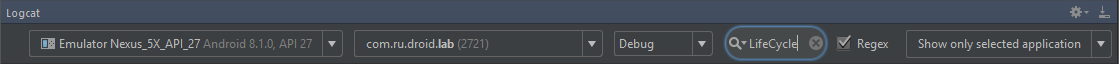
\includegraphics[scale=.7]{log.png}
\caption{Filter logs}
\label{fig:logfilt}
\end{figure}

Using \texttt{Log.d} we can monitor the lifecycle of the two activities found in listings \ref{listing:twoactxml} and \ref{listing:twoactjava} (the source code can be found \href{https://github.com/JonSteinn/AndroidDevelopment/tree/master/examples/lab3/lifecycle}{here}). You should try various scenarios of navigating between the apps as well as rotating the screen and using the Android back button.

\begin{lstlisting}[style=A_XML,caption={Two layouts for two activities},label={listing:twoactxml}]
<?xml version="1.0" encoding="utf-8"?>
<LinearLayout xmlns:android="http://schemas.android.com/apk/res/android"
    xmlns:tools="http://schemas.android.com/tools"
    android:layout_width="match_parent"
    android:layout_height="match_parent"
    android:orientation="vertical"
    android:gravity="center"
    tools:context="com.ru.droid.lab.MainActivity">
    <TextView
        android:layout_width="wrap_content"
        android:layout_height="wrap_content"
        android:text="Activity 1"/> <!-- move to res -->
    <Button
        android:layout_width="wrap_content"
        android:layout_height="wrap_content"
        android:onClick="gotoWithoutFinish"
        android:text="goto 2"/> <!-- move to res -->
    <Button
        android:layout_width="wrap_content"
        android:layout_height="wrap_content"
        android:onClick="gotoAndFinish"
        android:text="goto 2 and finish"/> <!-- move to res -->
</LinearLayout>

<?xml version="1.0" encoding="utf-8"?>
<LinearLayout xmlns:android="http://schemas.android.com/apk/res/android"
    xmlns:tools="http://schemas.android.com/tools"
    android:layout_width="match_parent"
    android:layout_height="match_parent"
    android:orientation="vertical"
    android:gravity="center"
    tools:context="com.ru.droid.lab.SecondActivity">
    <TextView
        android:layout_width="wrap_content"
        android:layout_height="wrap_content"
        android:text="Activity 2"/> <!-- move to res -->
    <Button
        android:layout_width="wrap_content"
        android:layout_height="wrap_content"
        android:onClick="gotoWithoutFinish"
        android:text="goto 1"/> <!-- move to res -->
    <Button
        android:layout_width="wrap_content"
        android:layout_height="wrap_content"
        android:onClick="gotoAndFinish"
        android:text="goto 1 and finish"/> <!-- move to res -->
</LinearLayout>

\end{lstlisting}

\begin{lstlisting}[style=A_Java,caption={Overriding on activity lifecycle callbacks for two activities},label={listing:twoactjava}]
public class MainActivity extends AppCompatActivity {
    @Override
    protected void onCreate(Bundle savedInstanceState) {
        super.onCreate(savedInstanceState);
        setContentView(R.layout.activity_main);
        Log.d("LifeCycle", "Activity 1: onCreate");
    }
    @Override
    protected void onStart() {
        super.onStart();
        Log.d("LifeCycle", "Activity 1: onStart");
    }
    @Override
    protected void onResume() {
        super.onResume();
        Log.d("LifeCycle", "Activity 1: onResume");
    }
    @Override
    protected void onPause() {
        super.onPause();
        Log.d("LifeCycle", "Activity 1: onPause");
    }
    @Override
    protected void onStop() {
        super.onStop();
        Log.d("LifeCycle", "Activity 1: onStop");
    }
    @Override
    protected void onDestroy() {
        super.onDestroy();
        Log.d("LifeCycle", "Activity 1: onDestroy");
    }
    public void gotoWithoutFinish(View view) {
        startActivity(new Intent(MainActivity.this, SecondActivity.class));
    }
    public void gotoAndFinish(View view) {
        startActivity(new Intent(MainActivity.this, SecondActivity.class));
        finish();
    }
}

public class SecondActivity extends AppCompatActivity {
    @Override
    protected void onCreate(Bundle savedInstanceState) {
        super.onCreate(savedInstanceState);
        setContentView(R.layout.activity_second);
        Log.d("LifeCycle", "Activity 2: onCreate");
    }
    @Override
    protected void onStart() {
        super.onStart();
        Log.d("LifeCycle", "Activity 2: onStart");
    }
    @Override
    protected void onResume() {
        super.onResume();
        Log.d("LifeCycle", "Activity 2: onResume");
    }
    @Override
    protected void onPause() {
        super.onPause();
        Log.d("LifeCycle", "Activity 2: onPause");
    }
    @Override
    protected void onStop() {
        super.onStop();
        Log.d("LifeCycle", "Activity 2: onStop");
    }
    @Override
    protected void onDestroy() {
        super.onDestroy();
        Log.d("LifeCycle", "Activity 2: onDestroy");
    }
    public void gotoWithoutFinish(View view) {
        startActivity(new Intent(SecondActivity.this, MainActivity.class));
    }
    public void gotoAndFinish(View view) {
        startActivity(new Intent(SecondActivity.this, MainActivity.class));
        finish();
    }
}
\end{lstlisting}


\subsection{Passing data between activities}
As we have already discussed, Intents are something of a bridge between activities. We used it to start a new activity but it can also be used to pass data between activities.

\begin{lstlisting}[style=A_Java]
Intent intent = new Intent(MainActivity.this, SecondActivity.class);
intent.put("SOME_KEY", "SOME_VALUE");
startActivity(intent);
\end{lstlisting}

The parameter we are using here is an instance of the current activity and a \texttt{.class} of the activity we want to lunch. This is called a reflection and is provides a way to get metadata on classes during runtime. The Intent constructor is overloaded so these are not the only options for parameters. We can use \texttt{getIntent()} to access the intent in the newly lunched activity and depending on the data type, there are various methods to access values given keys.

\begin{lstlisting}[style=A_Java]
Intent intent = getIntent();
String value = intent.getStringExtra("SOME_KEY");
\end{lstlisting}

In listings \ref{listing:loginxml} and \ref{listing:loginjava} the first activity has a simple login UI with validation (using a simple hard coded list of accepted username and passwords) and if successful, we proceed to the next activity passing along the username for a personal greeting. The source code can be found \href{https://github.com/JonSteinn/AndroidDevelopment/tree/master/examples/lab3/login}{here}.

\begin{lstlisting}[style=A_XML, caption={Layouts for simple login}, label={listing:loginxml}]
<resources>
    <string name="app_name">Lab</string>
    <string name="un_hint">Enter your username</string>
    <string name="pw_hint">Enter your password</string>
    <string name="login">Login</string>
    <string name="welcome">Welcome</string>
    <string name="required">Required</string>
    <string name="incorrect">Incorrect</string>
</resources>

<?xml version="1.0" encoding="utf-8"?>
<LinearLayout xmlns:android="http://schemas.android.com/apk/res/android"
    xmlns:tools="http://schemas.android.com/tools"
    android:layout_width="match_parent"
    android:layout_height="match_parent"
    android:orientation="vertical"
    android:gravity="center"
    tools:context="com.ru.droid.lab.MainActivity">
    <EditText
        android:id="@+id/username"
        android:layout_width="match_parent"
        android:layout_height="wrap_content"
        android:layout_marginLeft="15dp"
        android:layout_marginRight="15dp"
        android:ems="10"
        android:inputType="textPersonName"
        android:hint="@string/un_hint"/>
    <EditText
        android:id="@+id/password"
        android:layout_width="match_parent"
        android:layout_height="wrap_content"
        android:layout_marginLeft="15dp"
        android:layout_marginRight="15dp"
        android:ems="10"
        android:inputType="textPassword"
        android:hint="@string/pw_hint"/>
    <Button
        android:layout_width="match_parent"
        android:layout_height="wrap_content"
        android:layout_marginLeft="15dp"
        android:layout_marginRight="15dp"
        android:text="@string/login"
        android:onClick="attemptLogin"/>
</LinearLayout>

<?xml version="1.0" encoding="utf-8"?>
<LinearLayout xmlns:android="http://schemas.android.com/apk/res/android"
    xmlns:tools="http://schemas.android.com/tools"
    android:layout_width="match_parent"
    android:layout_height="match_parent"
    android:orientation="vertical"
    android:gravity="center"
    tools:context="com.ru.droid.lab.SecondActivity">
    <TextView
        android:id="@+id/welcome_text"
        android:layout_width="wrap_content"
        android:layout_height="wrap_content"/>
</LinearLayout>
\end{lstlisting}

\begin{lstlisting}[style=A_JAVA, caption={A very simple login}, label={listing:loginjava}]
public final class FakeDB {
    private static Map<String, String> usersAndPasswords = new HashMap<>();
    static {
        usersAndPasswords.put("Max", "abcd");
        usersAndPasswords.put("Mona", "1234");
        usersAndPasswords.put("Vladimir", "Vodka");
        usersAndPasswords.put("Nicole", "PV");
        usersAndPasswords.put("Alfred", "IC");
    }
    public static boolean doesExist(String un) {
        return usersAndPasswords.containsKey(un);
    }
    public static boolean correctPassword(String un, String pw) {
        return usersAndPasswords.containsKey(un) && usersAndPasswords.get(un).equals(pw);
    }
    private FakeDB() {}
}

public class MainActivity extends AppCompatActivity {
    private EditText username;
    private EditText password;

    @Override
    protected void onCreate(Bundle savedInstanceState) {
        super.onCreate(savedInstanceState);
        setContentView(R.layout.activity_main);

        this.username = (EditText)findViewById(R.id.username);
        this.password = (EditText)findViewById(R.id.password);
    }

    public void attemptLogin(View view) {
        String un = username.getText().toString();
        String pw = password.getText().toString();
        if (un.trim().length() == 0) {
            username.requestFocus();
            username.setError(getResources().getString(R.string.required));
        } else if (!FakeDB.doesExist(un)) {
            username.requestFocus();
            username.setError(getResources().getString(R.string.incorrect));
        } else if (pw.trim().length() == 0) {
            password.requestFocus();
            password.setError(getResources().getString(R.string.required));
        } else if (!FakeDB.correctPassword(un, pw)) {
            password.requestFocus();
            password.setError(getResources().getString(R.string.incorrect));
        } else {
            Intent intent = new Intent(this, SecondActivity.class);
            intent.putExtra("USER_NAME", un);
            startActivity(intent);
            finish();
        }
    }
}

public class SecondActivity extends AppCompatActivity {
    @Override
    protected void onCreate(Bundle savedInstanceState) {
        super.onCreate(savedInstanceState);
        setContentView(R.layout.activity_second);

        Intent intent = getIntent();
        String un = intent.getStringExtra("USER_NAME");

        String msg = getResources().getString(R.string.welcome) + ", " + un;
        ((TextView)findViewById(R.id.welcome_text)).setText(msg);
    }
}
\end{lstlisting}

We might also want to get data to other way around, from a lunched activity to the activity the lunched it. For that we can use \texttt{startActivityForResult()} and the callback method \texttt{onActivityResult()}. Suppose we have two activities A and B where A lunches B and expects results. A must use a unique id for starting the activity B for results and check if it matches when the callback is invoked. The activity B must set results before finishing which involves the intent of data and a result code (can be custom) which the activity A can also check for.\\

Listings \ref{listing:xmlforres} and \ref{listing:javaforres} show an app where the main activity contains just a single button which upon clicking starts the second activity for result. In the second activity there is an input field and a button for sending back the result (the text in the input field) and then destroying itself. The main activity then uses a callback to set the text of its button with the value passed by the second activity, given that the id and code match. The source code can be found \href{https://github.com/JonSteinn/AndroidDevelopment/tree/master/examples/lab3/activityforresult}{here}.

\begin{lstlisting}[style=A_XML, caption={Layout for start activity for result}, label={listing:xmlforres}]
<resources>
    <string name="app_name">Lab</string>
    <string name="msg_field">Enter message (no more than 6 chars)</string>
    <string name="send_back">send back</string>
    <string name="init_btn_msg">Click ME</string>
</resources>

<?xml version="1.0" encoding="utf-8"?>
<LinearLayout xmlns:android="http://schemas.android.com/apk/res/android"
    xmlns:tools="http://schemas.android.com/tools"
    android:layout_width="match_parent"
    android:layout_height="match_parent"
    android:orientation="vertical"
    android:gravity="center"
    tools:context="com.ru.droid.lab.MainActivity">
    <Button
        android:id="@+id/btn"
        android:layout_width="match_parent"
        android:layout_height="wrap_content"
        android:layout_margin="50dp"
        android:onClick="click"
        android:text="@string/init_btn_msg"/>
</LinearLayout>

<?xml version="1.0" encoding="utf-8"?>
<LinearLayout xmlns:android="http://schemas.android.com/apk/res/android"
    xmlns:tools="http://schemas.android.com/tools"
    android:layout_width="match_parent"
    android:layout_height="match_parent"
    android:orientation="vertical"
    android:gravity="center"
    tools:context="com.ru.droid.lab.SecondActivity">

    <EditText
        android:id="@+id/msg_id"
        android:layout_width="match_parent"
        android:layout_height="wrap_content"
        android:layout_margin="15dp"
        android:maxLength="6"
        android:textAlignment="center"
        android:hint="@string/msg_field"/>
    <Button
        android:layout_width="wrap_content"
        android:layout_height="wrap_content"
        android:text="@string/send_back"
        android:onClick="sendBackResults"/>
</LinearLayout>
\end{lstlisting}

\begin{lstlisting}[style=A_Java, caption={Start activity for result}, label={listing:javaforres}]
public class MainActivity extends AppCompatActivity {
    private static final int REQ_ID = 1111;

    @Override
    protected void onCreate(Bundle savedInstanceState) {
        super.onCreate(savedInstanceState);
        setContentView(R.layout.activity_main);
    }

    public void click(View view) {
        Intent intent = new Intent(this, SecondActivity.class);
        startActivityForResult(intent, REQ_ID);
    }

    @Override
    protected void onActivityResult(int requestCode, int resultCode, Intent data) {
        if (requestCode == REQ_ID) {
            if (resultCode == RESULT_OK) {
                String val = data.getStringExtra("MSG");
                ((Button) findViewById(R.id.btn)).setText(val);
            } else {
                Toast.makeText(this, "ERROR", Toast.LENGTH_SHORT).show();
            }
        }
    }
}

public class SecondActivity extends AppCompatActivity {

    @Override
    protected void onCreate(Bundle savedInstanceState) {
        super.onCreate(savedInstanceState);
        setContentView(R.layout.activity_second);
    }

    public void sendBackResults(View view) {
        Intent intent = new Intent();
        EditText msg = (EditText)findViewById(R.id.msg_id);
        intent.putExtra("MSG", msg.getText().toString());
        setResult(RESULT_OK, intent);
        finish();
    }
}
\end{lstlisting}

\section{Layout inflater}
Before we look into fragments, we will take a look at another way of re-using code using layout inflaters. Suppose we want to multiple instances of the same partial layout on our screen like can be seen in figure \ref{fig:infldem}, it would be very tedious to write seperate views and code for all of them, especially if they become complicated. 

\begin{figure}[H]
\centering
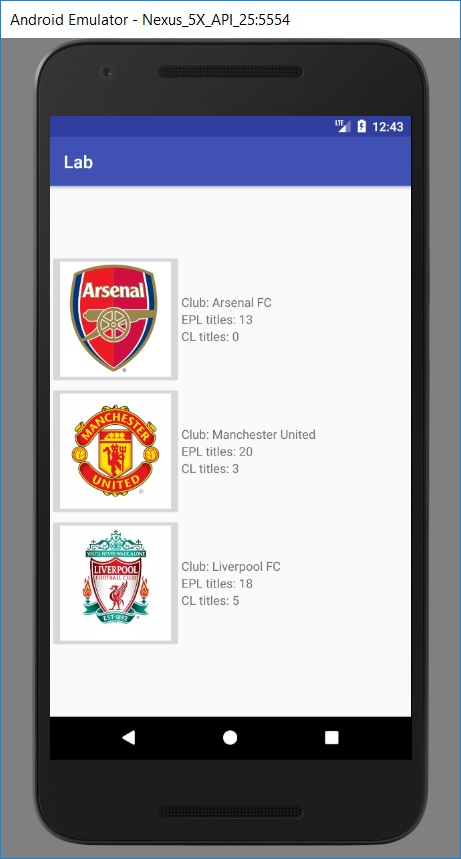
\includegraphics[scale=.5]{inflate_demo.png}
\caption{Same layout used 3 times with layout inflater}
\label{fig:infldem}
\end{figure}

To re-use a layout, we can use what is called a layout inflater. Start by creating a new layout resource file by right clicking on your layout folder and selecting \menu{New > New > Android resource file} and name it \texttt{team.xml}. In it we will create a layout for a single team as seen in figure \ref{fig:infldem}. The XML can be seen in listing \ref{listing:xmlinfldem}. Note that the main layout has an id but and some attributes set but has no children so nothing would be visible here unless we make it so in Java.

\begin{lstlisting}[style=A_XML, caption={XML for inflater demo}, label={listing:xmlinfldem}]
<!-- Activity's layout -->
<?xml version="1.0" encoding="utf-8"?>
<LinearLayout xmlns:android="http://schemas.android.com/apk/res/android"
    xmlns:tools="http://schemas.android.com/tools"
    android:id="@+id/root_view"
    android:layout_width="match_parent"
    android:layout_height="match_parent"
    android:orientation="vertical"
    android:gravity="center"
    tools:context="com.ru.droid.lab.MainActivity">
</LinearLayout>

<!-- team.xml -->
<?xml version="1.0" encoding="utf-8"?>
<LinearLayout xmlns:android="http://schemas.android.com/apk/res/android"
    android:id="@+id/team_outer_layout"
    android:layout_width="match_parent"
    android:layout_height="wrap_content"
    android:orientation="horizontal"
    android:gravity="center_vertical">
    <ImageButton
        android:id="@+id/team_img"
        android:layout_width="150dp"
        android:layout_height="150dp"
        android:scaleType="fitXY"/>
    <LinearLayout
        android:id="@+id/team_inner_layout"
        android:layout_width="wrap_content"
        android:layout_height="wrap_content"
        android:orientation="vertical">
        <TextView
            android:id="@+id/team_title"
            android:layout_width="wrap_content"
            android:layout_height="wrap_content"/>
        <TextView
            android:id="@+id/team_epl"
            android:layout_width="wrap_content"
            android:layout_height="wrap_content"/>
        <TextView
            android:id="@+id/team_cl"
            android:layout_width="wrap_content"
            android:layout_height="wrap_content"/>
    </LinearLayout>
</LinearLayout>

<!-- String with formats! -->
<resources>
    <string name="app_name">Lab</string>
    <string name="team_name">Club: %s</string>
    <string name="team_epl">EPL titles: %s</string>
    <string name="team_cl">CL titles: %s</string>
</resources>
\end{lstlisting}

In this example we have 3 figures in the drawable folder called \texttt{afc.jpg}, \texttt{lfc.jpg} and \texttt{mufc.jpg}. We also provide a fake database that gives us the option of iterating over all images.

\begin{lstlisting}[style=A_Java]
public final class FakeDB {
    private static Map<Integer, TeamInfo> imageDetail;
    private static void init() {
        if (imageDetail == null) {
            imageDetail = new HashMap<>();
            imageDetail.put(R.drawable.afc,
                    new TeamInfo("Arsenal FC", 13, 0));
            imageDetail.put(R.drawable.lfc,
                    new TeamInfo("Liverpool FC", 18, 5));
            imageDetail.put(R.drawable.mufc,
                    new TeamInfo("Manchester United", 20, 3));
        }
    }
    public static Iterable<Map.Entry<Integer, TeamInfo>> getAllImages() {
        init();
        return imageDetail.entrySet();
    }
}

public final class TeamInfo {
    private String name;
    private String eplTitles;
    private String clTitles;
    public TeamInfo(String name, int epl, int cl) {
        this.name = name;
        this.eplTitles = Integer.toString(epl);
        this.clTitles = Integer.toString(cl);
    }
    public String getName() {
        return this.name;
    }
    public String getEplTitles() {
        return this.eplTitles;
    }
    public String getClTitles() {
        return this.clTitles;
    }
}
\end{lstlisting}

Now we can implement our activity to populate its layout with inflated views created from our layout resource.

\begin{lstlisting}[style=A_Java, caption={Layout inflation in Java}, label={listing:javainfl}]]
public class MainActivity extends AppCompatActivity {

    @Override
    protected void onCreate(Bundle savedInstanceState) {
        super.onCreate(savedInstanceState);
        setContentView(R.layout.activity_main);
        populateLayout();
    }

    private void populateLayout() {
        LinearLayout root = (LinearLayout)findViewById(R.id.root_view);
        for (Map.Entry<Integer, TeamInfo> info : FakeDB.getAllImages()) {
            addNewTeam(root, info.getKey(), info.getValue());
        }
    }

    private void addNewTeam(LinearLayout parent,
                            final int img, final TeamInfo info) {

        // Create new view with inflate
        View team = View.inflate(this, R.layout.team, null);

        // Set button image source and on click listener
        ImageButton btn = (ImageButton)team.findViewById(R.id.team_img);
        btn.setImageResource(img);
        btn.setOnClickListener(new View.OnClickListener() {
            @Override
            public void onClick(View v) {
                Toast.makeText(MainActivity.this, info.getName(),
                        Toast.LENGTH_SHORT).show();
            }
        });

        Resources res = getResources();

        // Set club's name using resource string format
        TextView name = (TextView)team.findViewById(R.id.team_title);
        name.setText(res.getString(R.string.team_name, info.getName()));

        // Set club's epl title count using resource string format
        TextView epl = (TextView)team.findViewById(R.id.team_epl);
        epl.setText(res.getString(R.string.team_epl, info.getEplTitles()));

        // Set club's cl title count using resource string format
        TextView cl = (TextView)team.findViewById(R.id.team_cl);
        cl.setText(res.getString(R.string.team_cl, info.getClTitles()));

        // Add the view to our root view group
        parent.addView(team);

    }
}
\end{lstlisting}

Note that we are not using \texttt{findViewById} from our current instance but rather using the template view and searching for them within it. The source code for this example is available \href{https://github.com/JonSteinn/AndroidDevelopment/tree/master/examples/lab3/inflator}{here}.

\section{Fragments}
Fragments are a re-usable UI component that can be added to an activity. They are similar to activities in many ways, something like a smaller version of activities. They have their own layout and lifecycle although they do live and depend on activities, that is their state depends on the state of their activity. The lifecycle of a fragment can be seen in figure \ref{fig:flife}.

\begin{figure}[H]
\centering
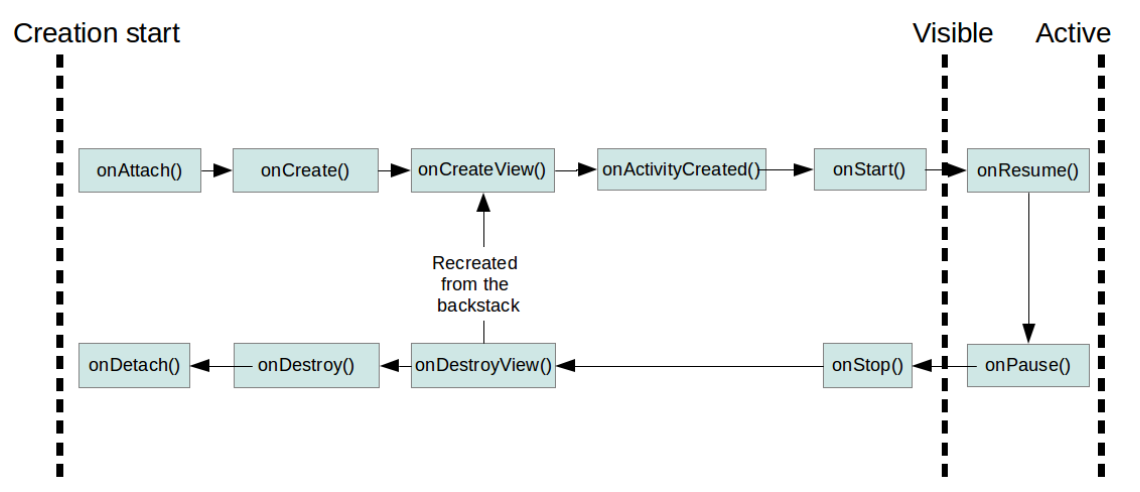
\includegraphics[scale=.75]{fragment_state_machine.png}
\caption{Fragment lifecycle}
\label{fig:flife}
\end{figure}

We will not go into much detail about the state or callbacks of a fragment. The \texttt{onCreateView} method must always be overwritten and it creates and returns the view hierarchy associated with the fragment. Another callback that we will have to use is \texttt{onActivityCreated} which is called when the parent activity has finished its own \texttt{onCreate} method.\\

Suppose we want to create a UI that is both suited for tablets or phones, or for both portrait and landscape mode on our phone. We could use a layout inflater or we could just remake the entire UI for both of them. We can also use fragments to create re-usable components that has all the logic and rendering for whatever we want to do, while the activity only looks at how to render the fragments. An example of such a scenario can be seen in figure \ref{fig:freuse} where we have a list of something and upon clicking, it shows us more details on what was selected. Here we could have one activity that has two different layouts depending on the mode, one displaying one fragment while the other displays two fragments.

\begin{figure}[H]
\centering
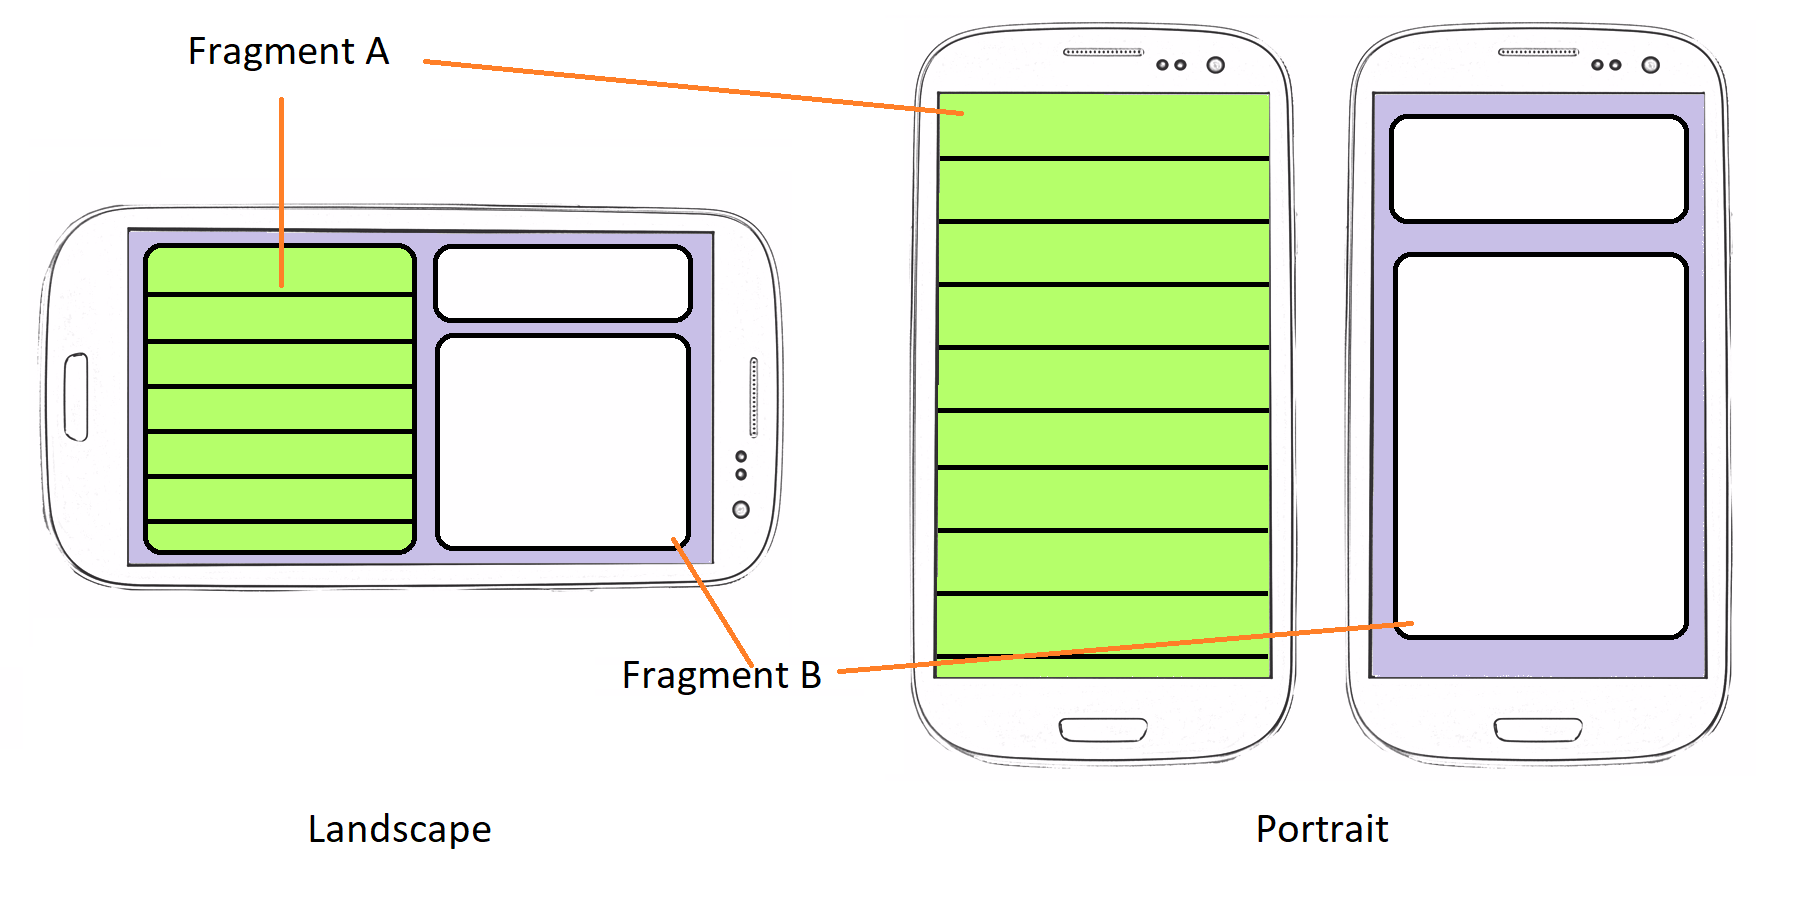
\includegraphics[scale=.4]{fragment_for_modes.png}
\caption{Re-usable fragments}
\label{fig:freuse}
\end{figure}

Lets start by creating a new resource file. Select layout as type, add orientation as a qualifier and set it to landscape and name the layout the same as your layout for your luncher activity. Android will automatically look for the landscape layout when it enter landscape mode.\\

Next we want to create to new fragments, \menu{File > New > Fragment > Fragment (Blank)}. You do not need to include fragment factory methods or include interface callbacks.\\

In listings \ref{listing:fragxml} and \ref{listing:javaxml} we provide a code (also available \href{www.TODO.com}{here}) for a simple app using fragments to support landscape and portrait mode. You can click on the box cover of a few video games and when you do you get a screenshot of the game in a new activity. If you however go to landscape mode and click a box cover, you get the screenshot on the same activity.

\begin{lstlisting}[style=A_XML, caption={XML for fragment example}, label={listing:fragxml}]
<!-- Fragment for choices -->
<LinearLayout xmlns:android="http://schemas.android.com/apk/res/android"
    xmlns:tools="http://schemas.android.com/tools"
    android:id="@+id/choose_root"
    android:layout_width="match_parent"
    android:layout_height="match_parent"
    android:orientation="vertical"
    android:gravity="center"
    tools:context="com.ru.droid.lab.fragments.ChooseFragment">
    <TextView
        android:layout_weight="0.1"
        android:layout_width="match_parent"
        android:layout_height="wrap_content"
        android:gravity="center"
        android:textSize="20sp"
        android:text="@string/vid90"/>

    <LinearLayout
        android:layout_weight="0.45"
        android:layout_height="0dp"
        android:layout_width="match_parent"
        android:gravity="center"
        android:orientation="horizontal">
        <ImageButton
            android:id="@+id/btn_mdk"
            android:src="@drawable/mdk"
            android:layout_height="wrap_content"
            android:layout_width="175dp"
            android:adjustViewBounds="true"
            android:scaleType="fitCenter"/>
        <ImageButton
            android:id="@+id/btn_carma"
            android:src="@drawable/carmageddon"
            android:layout_height="wrap_content"
            android:layout_width="175dp"
            android:adjustViewBounds="true"
            android:scaleType="fitCenter"/>
    </LinearLayout>

    <LinearLayout
        android:layout_weight="0.45"
        android:layout_height="0dp"
        android:layout_width="match_parent"
        android:gravity="center"
        android:orientation="horizontal">
        <ImageButton
            android:id="@+id/btn_jazz"
            android:src="@drawable/jazz_jackrabbit2"
            android:layout_height="wrap_content"
            android:layout_width="175dp"
            android:adjustViewBounds="true"
            android:scaleType="fitCenter"/>
        <ImageButton
            android:id="@+id/btn_dung"
            android:src="@drawable/dungeon_keeper"
            android:layout_height="wrap_content"
            android:layout_width="175dp"
            android:adjustViewBounds="true"
            android:scaleType="fitCenter"/>
    </LinearLayout>
</LinearLayout>

<!-- Fragment layout for screenshot -->
<LinearLayout xmlns:android="http://schemas.android.com/apk/res/android"
    xmlns:tools="http://schemas.android.com/tools"
    android:layout_width="match_parent"
    android:layout_height="match_parent"
    android:orientation="vertical"
    android:gravity="center"
    tools:context="com.ru.droid.lab.fragments.ScreenshotFragment">

    <TextView
        android:id="@+id/ss_title"
        android:layout_width="match_parent"
        android:layout_height="wrap_content"
        android:gravity="center"
        android:textSize="30sp"
        android:layout_weight="0.20"/>

    <ImageView
        android:id="@+id/ss_img"
        android:layout_margin="10dp"
        android:layout_width="match_parent"
        android:layout_height="0dp"
        android:layout_weight="0.8"/>

</LinearLayout>

<!-- Landscape layout for activity_main -->
<?xml version="1.0" encoding="utf-8"?>
<LinearLayout xmlns:android="http://schemas.android.com/apk/res/android"
    xmlns:tools="http://schemas.android.com/tools"
    android:orientation="horizontal"
    android:gravity="center"
    android:layout_width="match_parent"
    android:layout_height="match_parent">

    <fragment
        android:id="@+id/c_frag_land"
        android:name="com.ru.droid.lab.fragments.ChooseFragment"
        tools:layout="@layout/fragment_choose"
        android:layout_weight="0.5"
        android:layout_width="0dp"
        android:layout_height="match_parent">
    </fragment>

    <fragment
        android:id="@+id/ss_frag_land"
        android:name="com.ru.droid.lab.fragments.ScreenshotFragment"
        tools:layout="@layout/fragment_screenshot"
        android:layout_weight="0.5"
        android:layout_width="0dp"
        android:layout_height="match_parent">
    </fragment>
</LinearLayout>

<!-- Default layout for activity_main -->
<?xml version="1.0" encoding="utf-8"?>
<FrameLayout xmlns:android="http://schemas.android.com/apk/res/android"
    xmlns:tools="http://schemas.android.com/tools"
    android:id="@+id/frag_container"
    android:layout_width="match_parent"
    android:layout_height="match_parent"
    tools:context="com.ru.droid.lab.activities.MainActivity">
    <fragment
        android:id="@+id/c_frag"
        android:name="com.ru.droid.lab.fragments.ChooseFragment"
        tools:layout="@layout/fragment_choose"
        android:layout_width="match_parent"
        android:layout_height="match_parent">
    </fragment>
</FrameLayout>

<!-- Layout for screenshot activity -->
<?xml version="1.0" encoding="utf-8"?>
<FrameLayout xmlns:android="http://schemas.android.com/apk/res/android"
    xmlns:tools="http://schemas.android.com/tools"
    android:layout_width="match_parent"
    android:layout_height="match_parent"
    tools:context="com.ru.droid.lab.activities.ScreenshotActivity">
    <fragment
        android:id="@+id/ss_frag"
        android:name="com.ru.droid.lab.fragments.ScreenshotFragment"
        tools:layout="@layout/fragment_screenshot"
        android:layout_width="match_parent"
        android:layout_height="match_parent">
    </fragment>
</FrameLayout>
\end{lstlisting}

\begin{lstlisting}[style=A_Java, caption={Java for fragment example}, label={listing:javaxml}]
public class MainActivity extends AppCompatActivity {
    @Override
    protected void onCreate(Bundle savedInstanceState) {
        super.onCreate(savedInstanceState);
        setContentView(R.layout.activity_main);
    }
}

public class ScreenshotActivity extends AppCompatActivity {
    @Override
    protected void onCreate(Bundle savedInstanceState) {
        super.onCreate(savedInstanceState);
        setContentView(R.layout.activity_screenshot);
        // If we are in the second activity when we rotate our phone to
        // landscape mode, we finish it and return to the main activity
        if (getResources().getConfiguration().orientation
                == Configuration.ORIENTATION_LANDSCAPE) {
            finish();
        }
    }
}

public class Data {
    private int screenShotId;
    private String screenShotTitle;
    public Data(int id, String title) {
        screenShotId = id;
        screenShotTitle = title;
    }
    public int getScreenShotId() {
        return screenShotId;
    }
    public String getScreenShotTitle() {
        return screenShotTitle;
    }
}

public final class FakeDB {
    private static Map<Integer, Data> screenshotIDs;
    private static void init() {
        if (screenshotIDs == null) {
            screenshotIDs = new HashMap<>();
            screenshotIDs.put(R.id.btn_carma, new Data(R.drawable.carmageddon_ss, "Carmageddon"));
            screenshotIDs.put(R.id.btn_jazz, new Data(R.drawable.jazz_jackrabbit2_ss, "Jazz Jackrabbit 2"));
            screenshotIDs.put(R.id.btn_mdk, new Data(R.drawable.mdk_ss, "MDK"));
            screenshotIDs.put(R.id.btn_dung, new Data(R.drawable.dungeon_keeper_ss, "Dungeon Keeper"));
        }
    }
    public static Iterable<Integer> getButtons() {
        init();
        return screenshotIDs.keySet();
    }
    public static Data getScreenshot(int id) {
        init();
        return screenshotIDs.get(id);
    }
    private FakeDB() {}
}

public class ChooseFragment extends Fragment {
    public ChooseFragment() {}

    @Override
    public View onCreateView(LayoutInflater inflater, ViewGroup container,
                             Bundle savedInstanceState) {
        return inflater.inflate(R.layout.fragment_choose, container, false);
    }

    @Override
    public void onActivityCreated(Bundle savedState) {
        super.onActivityCreated(savedState);
        setOnClickListeners(getActivity());
    }

    private void setOnClickListeners(final Activity a) {
        for (Integer btnId : FakeDB.getButtons()) {
            a.findViewById(btnId).setOnClickListener(v -> imageClick(v, a));
        }
    }

    private void imageClick(View v, Activity a) {
        Data d = FakeDB.getScreenshot(v.getId());
        if (portraitMode(a)) {
            Intent intent = new Intent(a, ScreenshotActivity.class);
            intent.putExtra("SCREENSHOT_ID", d.getScreenShotId());
            intent.putExtra("SCREENSHOT_TITLE", d.getScreenShotTitle());
            a.startActivity(intent);
        } else {
            ScreenshotFragment ssf = (ScreenshotFragment)getFragmentManager()
                    .findFragmentById(R.id.ss_frag_land);
            ssf.setScreenShot(a, d.getScreenShotId(), d.getScreenShotTitle());
        }
    }

    private boolean portraitMode(Activity a) {
        return a.getResources().getConfiguration().orientation
                == Configuration.ORIENTATION_PORTRAIT;
    }
}

public class ScreenshotFragment extends Fragment {
    public ScreenshotFragment() {}

    @Override
    public View onCreateView(LayoutInflater inflater, ViewGroup container,
                             Bundle savedInstanceState) {
        return inflater.inflate(R.layout.fragment_screenshot, container, false);
    }

    @Override
    public void onActivityCreated(Bundle savedState) {
        super.onActivityCreated(savedState);

        Activity a = getActivity();
        Intent i = a.getIntent();
        int id = i.getIntExtra("SCREENSHOT_ID", -1);
        String title = i.getStringExtra("SCREENSHOT_TITLE");
        if (id != -1 && title != null) setScreenShot(a, id, title);
    }

    public void setScreenShot(Activity a, int id, String title) {
        ((ImageView)a.findViewById(R.id.ss_img)).setImageResource(id);
        ((TextView)a.findViewById(R.id.ss_title)).setText(title);
    }
}
\end{lstlisting}

\section{Assignment}
TODO: make template and better description:
%Task: Phonebook with add_new and view_details. Add_new can be a seperate activity in both landscape_and_portrait and shared between them. List of people and view must be in fragments and with similar UI as the example above. People are free to write static containers to store what they need.
